%%%%%%%%%%%%%%%%%%%%%%%%%%%%%%%%%%%%%%%%%%%%%%%%%%%%%%%%%%%
%
%		Relazione del Mid Term di Programmazione Avanzata
%
%				    Nicola Corti - 2012
%
%%%%%%%%%%%%%%%%%%%%%%%%%%%%%%%%%%%%%%%%%%%%%%%%%%%%%%%%%%%
\documentclass[a4paper,11pt]{book} 
\usepackage{graphicx}
\usepackage{amssymb}
\usepackage{vmargin}
\usepackage[italian]{babel} 
\usepackage[latin1]{inputenc}
\usepackage{listings}
\usepackage[usenames,dvipsnames,svgnames,table]{xcolor}
\usepackage{amsthm}
\usepackage{amsmath}
\usepackage{qtree}
%\usepackage{parskip}




\lstset{
basicstyle=\footnotesize\ttfamily,
keywordstyle=\color{MidnightBlue}\bfseries,
identifierstyle=\color{Black},
commentstyle=\color{Green}\itshape,
stringstyle=\color{Red}\ttfamily,
showstringspaces=false,
numbers=left, numberstyle=\tiny,
stepnumber=1, numbersep=10pt,
tabsize=4,
framexleftmargin=5mm, rulesepcolor=\color{Gray},
frame=tb,
%backgroundcolor=\color{GrigioChiaro},
language={C},
%mathescape=true,
%fontadjust=true,
%breaklines=true,breakatwhitespace=true,breakautoindent
}

\title{Appunti di Algoritmica 2}
\author{Nicola Corti - 454413 \\Corso di Laurea Magistrale in Informatica - Universit\`a di pisa}
\date{28 Novembre 2012}

 
\begin{document}

\setlength{\parskip}{0.10in}

\maketitle

\tableofcontents

\part{Randomization, hashing and data streaming}

\chapter{Data Streaming Model}

Nel modello del data streaming dobbiamo analizzare grosse quantit\`a di dati e non ci possiamo permettere di memorizzarli, ma dobbiamo memorizzarli in spazio polilogaritmico ed effettuare una singola scansione dello stream.

Questo modello ha subito una notevole evoluzione negli ultimi anni, specialmente perch\`e presenta molte applicazioni concrete:
\begin{enumerate}
\item Analisi del traffico in un router
\item Database e log delle query effettuate
\item Gestione delle telefonate
\end{enumerate}

In questo contesto, semplici problemi possono diventare molto difficili, inoltre solo alcuni problemi possono essere risolti facilmente in modo deterministico, ecco alcuni esempi:

\paragraph{Esempio 1} Trovare il massimo di uno stream di dati, sono necessari solamente $O(\log m)$ bit per memorizzare il massimo attuale.

\paragraph{Esempio 2} Trovare l'elemento mancante in uno stream che rappresenta una permutazione da 1 a n, dove un elemento \`e mancante: utilizzando la formula $$\sum_{e \in [1 \cdots n]} e = \frac{n(n+1)}{2}$$ ed effettuare delle sottrazioni per trovare il numero mancante, ma occuperemo $2 \log  m$ bits.

Possiamo invece utilizzare l'operazione di \textsf{XOR} ($\oplus$) ed utilizzare $\log m$ bit.

\section{Nozioni di probabilit\`a}

Prima di procedere nell'analisi di metodologie per affrontare il modello del data streaming sono necessarie alcune nozioni di probabilit\`a:
\begin{enumerate}
\item K-Wise Indipendence
\item Markov's Inequality
\item Chernoff's Bounds
\end{enumerate}

\subsection{K-Wise Indipendence}

Partiamo dal concetto del K-Wise indipendence per delle variabili aleatorie e definiamo dapprima il K-Wise limited indipendence:

\subsubsection{K-Wise Limited Indipendence}

Siano $X_1, X_2, \cdots, X_n$ variabili aleatorie e definiamo con $S_i = \mbox{support}(X_i)$ come il loro insieme di supporto, ovvere come l'insieme di valori che possono assumere le varie $X_i$.

Tali variabili aleatorie si dicono K-Wise indipendent se $\forall$ scelta di $i_1 < i_2 < \cdots < i_k \in [n]$ e $a_{i_j} \in S_{i_j}$ succede che:
$$\Pr[X_{i_1} = a_{i_1} \wedge X_{i_2} = a_{i_2} \wedge \cdots \wedge X_{i_k} = a_{i_k}] = \Pr[X_{i_1} = a_{i_1}] \times \Pr[X_{i_2} = a_{i_2}] \times \cdots \times \Pr[X_{i_k} = a_{i_k}] $$

Ne seguen facilmente che $$E[X_{i_1}, X_{i_2}, \cdots, E_{i_k}] = E[X_{i_1}] \times E[X_{i_2}] \times \cdots \times E[X_{i_k}] $$

Possiamo adesso estendere il concetto ad una famiglia di funzioni hash:

\subsubsection{Hash K-wise Indipendence}

Definiamo come $\{ h \}_{h \in H}$ una famiglia di funzioni hash $[n] \rightarrow [b]$ che supponiamo essere uniformamente distribuita, ovvero che $$ \Pr[h \in H] = \frac{1}{|H|}$$

Diremo che la famiglia H di funzioni hash \`e K-wise indipendente se succede che per ogni scelta di $x_1 < x_2 < \cdots < x_k \in [n], b_1 < b_2 < \cdots < b_k \in [b]$ succede che 
$$\Pr_{h \in H}[h(x_1) = b_1 \wedge \cdots \wedge h(x_k) = b_k] = \Pr_{h \in H}[h(x_1) = b_1] \times \cdots \times \Pr_{h \in H}[h(x_k) = b_k]$$

\paragraph{Esempio}

Consideriamo una famiglia di funzioni hash della seguente forma: $$h(x) = a_0 + a_1 x + a_2 x^2 + \cdots + a_{k-1} x^{k-1}$$ $$ a_i \in F \mbox{finite field}$$

Notiamo che una funzione risulta facilmente identificabile memorizzando i coefficienti $(a_0, a_1, a_2, \cdots, a_n)$ per cui possiamo cacolare facilmente la cardinalit\`a della famiglia di funzioni hash come $|H| = |F|^K$

Notiamo allora che ci sono $|F|^{k-1}$ funzioni hash che risolvono l'equazione $h(x_i) = b_i$ del tipo $$a_0 = b_i - a_1 x_i - a_2 x_i^{2} - \ldots - a_k x_i^{k}$$

Succede dunque che:
$$\underbrace{\Pr_{h \in H}[h(x_1) = b_1 \wedge \cdots \wedge h(x_k) = b_k]}_{\frac{1}{|F|^K}} = \underbrace{\Pr_{h \in H}[h(x_1) = b_1]}_{\frac{|F|^{K-1}}{|F|^K} = \frac{1}{|F|}} \times \cdots \times \Pr_{h \in H}[h(x_k) = b_k]$$

\subsection{Markov's Inequality}

Sia $X$ una variabile aleatoria $ \geq 0$ e sia $a \in \mathbb{R}, a > 0$ allora vale: $$\Pr[X \geq a] \leq \frac{\mathbb{E}[X]}{a}$$

\begin{proof}
In questa dimostrazione useremo le variabili indicatrici:
$$ I = \begin{cases} 
0 & \mbox{se } X < a \\
1 & \mbox{se } X \geq a \\
\end{cases} $$

Proviamo a calcolare il valore atteso della variabile indicatrice:
\begin{eqnarray}
\mathbb{E}[I] & = & 0 \cdot \Pr[I = 0] + 1 \cdot \Pr[I = 1] \nonumber \\
& = & 1 \cdot \Pr[I = 1] \nonumber \\
& = & \Pr[X \geq a] \nonumber \\
\end{eqnarray}
Adesso notiamo che $aI \leq X$:
\begin{itemize}
\item $X < a \Rightarrow I = 0$
\item $X \geq a \Rightarrow aI = a, a \leq X$
\end{itemize}
Adesso utilizzando i due fatti appena esaminati:
\begin{eqnarray}
\mathbb{E}[X] & \geq & \mathbb{E}[aI] \nonumber \\
& = & a \cdot \mathbb{E}[I] \nonumber \\
& = & a \cdot \Pr[X \geq a] \nonumber \\
\end{eqnarray}

Dividiamo per $a$ che ricordiamo essere reale positivo ed abbiamo dimostrato la disuguglianza di Markov.

\end{proof}

\subsection{Chernoff's Bounds}

Siano $Y_1, Y_2, \ldots, Y_r$ variabili aleatorie indipendenti ed equamente distribuite tali che $$\Pr[Y_j = 1] = p \quad \Pr[Y_j = 0 = 1-p$$
Definiamo inoltre: $$ Y = \sum_{j=1}^{r} Y_j \quad \mu = \mathbb{E}[Y] = \sum_{j=1}^{r}[Y_j] = rp$$ Allora possiamo effettuare la seguente stima anche detta Chernoff's Bound
$$\forall \lambda > 0 \quad \Pr[Y \geq (1+\lambda)\mu] < \left( \frac{e^{\lambda}}{(1+\lambda)^{1+\lambda}}\right)^{\mu}$$

\chapter{Count-min Sketch}

Descriviamo adesso il modello del count-min sketch (presentato da G. Cormode \& S. Muthukrishnan) che ci permette di approssimare le frequenze degli elementi in uno stream. 

Supponiamo di $n$ elementi distinti che possono occorrere nello stream, noi vorremmo calcolare $F[i]$, ovvero il numero di volte che un elemento $i$ occorre nello stream.

Le operazioni di base a nostra disposizione sono $F[i]++$ e $F[i]--$ ed andremo a calcolare $\tilde{F}[i]$ ovvero una versione approssimata di $F[i]$. Ricordiamoci che abbiamo a disposizione soltanto spazio $O(\log n)$ e non possiamo permetterci di memorizzare $F[i]$ per esteso. Inoltre operiamo sotto il seguente invariante:

\textbf{Invariante:} $F[i] \geq 0$

Ci accontenteremo di calcolare  $\tilde{F}[i]$ tale che 
$$\forall i \; F[i] \leq \underbrace{\tilde{F}[i] \leq F[i] + \varepsilon ||F||}_{\mbox{con prob.} \; \leq 1-\delta}$$

Dove $\varepsilon \geq 1 $ rappresenta il parametro di approssimazione, ovvero quanto vogliamo approssimare il risultato e $\delta \geq 0$ rappresenta il parametro di errore, indica di quanto stiamo sbagliando il risultato.

Infine indichiamo con $||F||$ la norma del vettore $F$ e la calcoliamo come $$||F|| = \sum_{x \in [n]} F[x]$$

\section{Algoritmo}

Il seguente \`e l'algoritmo per inizializzare e utilizzare il count-min sketch:

\begin{enumerate}
\item Definiamo $r = \log_2 \frac{1}{\delta}$ e $c = \frac{e}{\varepsilon}$, che saranno le dimensioni del nostro count-min sketch ($e$ \`e la costante di eulero).

\item Definiamo $T$ come un tabella di dimensioni $r \times c$ formata da contatori inizialmente settati a 0:

\begin{center}
\begin{tabular}{p{0.5cm}|p{0.5cm}|p{0.5cm}|p{0.5cm}|p{0.5cm}|p{0.5cm}|p{0.5cm}|}
\multicolumn{1}{c}{} &
\multicolumn{1}{c}{1} &
\multicolumn{1}{c}{2} &
\multicolumn{1}{c}{$\ldots$} &
\multicolumn{1}{c}{$\ldots$} &
\multicolumn{1}{c}{$\ldots$} &
\multicolumn{1}{c}{c} \\
\cline{2-7}
1 & & & & & &  \\
\cline{2-7}
2 & & & & & &  \\
\cline{2-7}
$\vdots$ & & & & & &  \\
\cline{2-7}
$\vdots$ & & & & & &  \\
\cline{2-7}
r & & & & & &  \\
\cline{2-7}
\end{tabular}
\end{center}

\item Si scelga una famiglia $H$ di funzioni hash che siano 2-wise independent. Ad esempio potremmo scegliere come famiglia la seguente $$h \in H \Leftrightarrow h(x) = (((ax + b) mod\; p )mod\; c)+1$$

\item Si scelgano $r$ funzioni hash $h_1, h_2, \ldots, h_r$ in modo uniforme ed indipendente dalla famiglia di funzioni hash $H$.

\item Preso un elemento $i$, associamo ad essi $r$ contatori, in modo che per ogni riga vi sia un elemento associato ad i, li scegliamo nel modo seguente: $$T(1, h_1(i)), T(2, h_2(i)), \ldots, T(r, h_r(i))$$.

Ovviamente succede che per due elementi $i \neq i'$ ci siano delle collisioni.

\item Eseguiamo le operazioni del modo seguente:
\begin{itemize}
\item $F[i]++ \Rightarrow$ incrementiamo di uno tutte le caselle associate all'elemento $i$, ovvero effettuaimo la seguente operazione $T(j, h_j (i))++ \forall j = 1, 2, \ldots, n$.
\item $F[i]-- \Rightarrow$ decrementiamo di uno tutte le caselle associate all'elemento $i$, ovvero effettuaimo la seguente operazione $T(j, h_j (i))++ \forall j = 1, 2, \ldots, n$.
\end{itemize}

\item Restituiamo l'approssimazione di $F[i]$ come il minimo valore assunto dalle caselle associate: $$\tilde{F}[i] = \min_{1 \leq j \leq r}T(j, h_j (i))$$

\end{enumerate}

\section{Dimostrazione}

Procediamo adesso a dimostrare le propriet\`a del count-min sketch

\paragraph{Fatto 1} Lo spazio occupato \`e $O(r \cdot c) = O(\varepsilon^{-1} \log \delta^{-1})$ parole di memoria, dove ogni parola di memoria pu\`o memorizzare $||F||$

\begin{proof}
Ogni contatore contiene un intero appartenente ad $\left[||F||\right]$
\end{proof}

\paragraph{Fatto 2} $F[i] \leq \tilde{F}[i]$

\begin{proof}
Per dimostrare questo fatto dobbiamo prima introdurre una variabile indicatrice che ci indica se c'\`e stata una collisione per una specifica riga, dati 2 elementi:$$ I_{j,i,k} = \begin{cases} 1 & \mbox{se } k \neq i \wedge h_j (i) = h_j (k) \\ 0 & \mbox{altrimenti} \\ \end{cases} $$

Definiamo supponiamo che abbiamo preso come approssimazione la $j-esima$ colonna: $$T(j, h_j (i)) = \tilde{F}[i]$$

Per il modo in cui abbiamo costruito il nostro count-min sketch allora $\exists i_1, i_2, \ldots, i_f $ elementi dello stream tali che uno di loro \`e $i$ e che hanno contribuito tutti ad incrementare il valore della casella considerata: $$T(j, h_j (i)) = \sum_{l = 1}^{f} F[i_l] = F[i] + X_{ji}$$

Dove $X_{ji}$ rappresenta la ``sporcizia'', ovvero l'eccesso dovuto alla presenza di collisioni sui contatori del count-min sketch. Per come l'abbiamo costruito vale che $X_{ji} \geq 0$, per cui il fatto risulta banalmente dimostrato.

\end{proof}


\paragraph{Osservazione 1} Osserviamo facilmente che possiamo espriemere la ``sporcizia'' nel modo seguente: $$X_{ji} = \sum_{k=1}^{n} I_{j,i,k} F[k]$$ dato che $X_{ij}$ vale 1 solamente quando c'\`e stata una collisione fra il nostro elemento $i$ e un altro elemento dello stream $k$.

\paragraph{Osservazione 2} Possiamo dimostrare che: $$ \mathbb{E}[I_{j,i,k}] = \frac{\varepsilon}{e}$$
\begin{proof}
\begin{eqnarray}
\mathbb{E}[I_{j,i,k}] & = & 0 \cdot \Pr[I_{j,i,k} = 0] + 1 \cdot \Pr[I_{j,i,k} = 1] \nonumber \\
& = & \Pr[I_{j,i,k} = 1] \nonumber \\
& = & \Pr\left[\exists a \in [c] : k \neq i \wedge h_j (i) = a \wedge  h_j (k) = a \right] \nonumber \\
& = & \Pr\left[\bigcup{a \in [c]} : k \neq i \wedge h_j (i) = a \wedge  h_j (k) = a \right] \nonumber \\
& = & \sum_{a \in [c]}\Pr\left[k \neq i \wedge h_j (i) = a \wedge  h_j (k) = a \right] \nonumber \\
& = & \sum_{a \in [c]}\underbrace{\Pr[h_j (i) = a]}_{1/c} \times \underbrace{\Pr\left[k \neq i \wedge  h_j (k) = a \right]}_{\mbox{``circa''} 1/c} \nonumber \\
& = & \sum_{a \in [c]}\frac{1}{c^2} = \frac{1}{c} = \frac{\varepsilon}{e} \nonumber
\end{eqnarray}
\end{proof}

Notiamo come nel penultimo passaggio si sia usata la probabilit\`a che $h_j$ \`e 2-Wise indipendent. Inoltre notiamo come il secondo termine sia circa $1/c$ dato che con la prima disuguaglianza escludiamo uno dei valori del dominio.

\paragraph{Fatto 3} $\tilde{F}[i] \leq F[i] + \varepsilon ||F|| $ con probabilit\`a $ \geq 1 - \delta$.

\begin{proof}
Al solito poniamo $\tilde{F}[i] = F[i] + X_{ij}$ dove $X_{ij} \geq 0$ \`e la solita ``sporcizia''.

Calcoliamo dapprima il valore atteso della sporcizia: 
$$\mathbb{E}[X_{ij}] = \mathbb{E}\left[\sum_{k=1}^{n} I_{j,i,k} F[k]\right] = \sum_{k=1}^{n} \mathbb{E}\left[I_{j,i,k} F[k]\right] \leq \sum_{k=1}^{n}\left(F[k] \cdot \underbrace{\mathbb{E}\left[I_{j,i,k}\right]}_{\varepsilon /e} \right) = $$
$$= \sum_{k=1}^{n}(F[k] \cdot \frac{\varepsilon}{e}) = \frac{\varepsilon}{e}||F||$$

Che equivale a dire che $e \mathbb{E}[X_{ij}] = \varepsilon ||F||$.

Con queste premesse calcoliamo:
\begin{eqnarray}
 \Pr[\tilde{F}[i] > F[i] + \varepsilon ||F||] & \leq & \delta \nonumber \\
 \Pr[\forall j \; F[i] + X_{ij} > F[i] + \varepsilon ||F||] & \leq & \delta \nonumber \\
 \Pr[\forall j \; X_{ij} > \varepsilon ||F||] & \leq & \delta \nonumber \\
 \Pr[\forall j \; X_{ij} > e \mathbb{E}[X_{ji}] & \leq & \delta \nonumber \\
 \Pr[X_{1i} > e \mathbb{E}[X_{1i}]] \times \ldots \times \Pr[X_{ri} > e \mathbb{E}[X_{ri}]] & \leq & \delta \nonumber 
\end{eqnarray}

Notiamo che l'ultimo passaggio si basa sul fatto che le $h_1, \ldots h_r$ funzioni hash sono scelte in modo indipendente e uniforme. Adesso approssimiamo un singolo termine con la disuguaglianza di Markov: $$\Pr[X_{ji} > e \mathbb{E}[X_{ji}]] \leq \frac{\mathbb{E}[X_{ji}]}{e \mathbb{E}[X_{ji}]} = \frac{1}{e} < \frac{1}{2} $$ 

Detto questo riscriviamo: $$ \Pr[X_{1i} > e \mathbb{E}[X_{1i}]] \times \ldots \times \Pr[X_{ri} > e \mathbb{E}[X_{ri}]] < \left(\frac{1}{2} \right)^r = \left(\frac{1}{2}\right)^{\log_2 \frac{1}{\delta}} = $$
$$ =  2^{-1} \log_{2} \delta^{-1} = \log_2 (\delta^{-1})^{2^{-1}} = \delta$$
\end{proof}

\section{Space Lower Bound}

Se consideriamo il problema del count-min sketch, notiamo che possiamo calcolare un limite inferiore per lo spazio necessario: $\Omega(1/\varepsilon$).

Per verificare questo limite inferiore dobbiamo introdurre alcuni concetti di \emph{communication complexity}
\begin{enumerate}
\item Definiamo dapprima l'\emph{INDEX problem}
\item Riduciamo l'\emph{INDEX problem} al calcolo di $\tilde{F}[i]$ 
\end{enumerate}

\subsection{Communication Complexity}

I problemi di communication complexity si presentano nel modo seguente: siano A (Alice) e B (Bob) due soggetti che devono comunicare fra di loro.
\begin{itemize}
\item Alice \`e in possesso di una sequenza di bit $x$
\item Bob \`e in possesso di una sequenza di bit $y$
\item L'obiettivo \`e che uno dei due soggetti riesca a calcolare una funzione $f(x,y)$ utilizzando il minor numero di bit per le comunicazioni possibile.
\end{itemize}

\subsection{L'\emph{INDEX problem}}

L'\emph{INDEX problem} rappresenta un particolare problema di communication complexity cos\`i definito:
\begin{itemize}
\item Alice \`e in possesso di una sequenza di bit $x \in \{0,1\}^n$
\item Bob \`e in possesso di una sequenza di bit $y \in \{0,1\}^{\log_2 n}$ ovvero \`e in possesso di un bit indica una posizione nella sequenza di Alice.
\item La funzione da calcolare \`e $f(x,y) = x_y$ ovvero conoscere il bit in posizione.
\item La comunicazione deve essere \emph{one round} da Alice a Bob, deve essere inviato cio\`e un solo messaggio.
\item Bob vuole calcolare $f(x,y)$ con $\Pr > 1/2$.
\end{itemize}
Notiamo che nel caso in cui la probabilit\`a sia $= 1/2$ allora il problema si risolve banalmente tirando una moneta e considerando il risultato.

Ci chiediamo allora quanti bit deve mandare Alice a Bob: deve mandare $m$ bit dove $$m \geq n(1-H(p))$$
Dove $H(p)$ rappresenta l'entropia cos\`i definita: $$H(p) = -p \log_2 p - (1-p) \log_2 (1-p)$$

Notiamo infine che $$n\underbrace{(1 - H(p))}_{0 < \ldots < 1} = \Omega(n) \mbox{bits}$$ Alice deve mandare essenzialmente buona parte del messaggio.

\subsection{Dimostrazione del lower bound}

Per dimostrare il nostro lower bound relativo allo spazio istanziamo l'\emph{INDEX problem} al caso del count-min sketch:

\begin{proof}
Istanziamo un \emph{INDEX problem} e scegliamo $\varepsilon$ tale che $n = \frac{1}{\varepsilon}$ ed inoltre $|x| = n$ ovvero $n$ \`e la dimensione dello stream dell'\emph{INDEX problem}.

Definiamo inoltre $$F\left[1\ldots\frac{1}{\varepsilon}\right] : F[i] = \begin{cases}
2 & \mbox{se } x[i] = 1 \\
0 & \mbox{se } x[i] = 0 \\
\end{cases}$$

Notiamo che stiamo amplificando i valori della $F[i]$ in modo da poter distinguere successivamente fra $\tilde{F}[i]$ e $F[i]$. 

Restringiamo l'insieme delle possibili stringhe del tipo $F\left[1\ldots\frac{1}{\varepsilon}\right]$ solamente a quelle tali che $\#2 = \#0 = n/2$ che risultano essere in numero pari a $\sum^n \binom{n}{n/2}$; questa restrizione ci servir\`a per calcolare in modo semplice la norma del vettore $F$, e vediamo che applicare questa restrizione \`e lecito dato che la funzione binomiale $\binom{n}{k}$ ha il suo punto di massimo in $k= n/2$. 

Cos\`i facendo risulta $$||F|| = 2 \times \frac{n}{2} = \frac{1}{\varepsilon}$$.

Il count-min sketch ci dice che \begin{eqnarray}
F[i] & \leq & \tilde{F[i]} \leq F[i] + \varepsilon||F|| \nonumber \\
F[i] & \leq & \tilde{F[i]} \leq F[i] + 1 \nonumber \\
\end{eqnarray}

Dato che abbiamo amplificato $F[i]$ che pu\`o valere solamente 0 o 2, possiamo risalire al valore di $F[i]$ partendo da $\tilde{F}[i]$, quindi applicando il risultato calcolato per l'\emph{INDEX problem} possiamo determinare che: $$\mbox{space}\left(\tilde{F}\left[1\ldots\frac{1}{\varepsilon}\right]\right) = \Omega(n) = \Omega(1/\varepsilon)$$

\end{proof}

\chapter{Esercizi sul Count-min sketch}

In questo capitolo mostriamo alcuni esercizi e applicazioni del count-min sketch visto in precedenza.

\section{Rimozione dell'invariante}

\`E possibile rimuovere l'invariante sul count-min sketch che avevamo imposto in precendenza, ovvero: 

\textbf{Invariante:} $F[i] \geq 0$

Cos\`i facendo dobbiamo per\`o ridefinire $\tilde{F}[i]$ come il mediano fra i valori dei contatori ovvero $$\tilde{F}[i] = \mbox{median}_{0 \leq j \leq r} \; T(j, h_j (i))$$

Rimuovendo l'invariante possiamo dimostrare, usando i Chernoff's Bound che vale la seguente relazione: $$F[i] - 3\varepsilon||F|| \leq \tilde{F}[i] \leq F[i] + 3\varepsilon||F||$$
$$ \mbox{con} \; p \geq 1 - \delta^{1/4}$$

che riscrivendo $\tilde{F}[i] = F[i] + X_{ij}$ equivale a dire che:
$$- 3\varepsilon||F|| \leq X_{ij} \leq + 3\varepsilon||F||$$
ovvero
$$ |X_{ij}| \leq 3 \varepsilon ||F||$$

\begin{proof}
Applichiamo dapprima la Markov inequality:
$$ \Pr[|X_{ij}| \geq 3 \varepsilon ||F||] < \frac{\overbrace{\mathbb{E}[|X_{ij}|]}^{\varepsilon / e||F||}}{3 \varepsilon ||F||} < \frac{1}{3e} < \frac{1}{8	}$$

Definiamo adesso una variabile indicatrice che vale 1 se il contatore selezionato non rispetta il vincolo che stiamo cercando di dimostrare:
$$ Y_j = \begin{cases} 1 & \mbox{se} \; |X_{ij}| > 3\varepsilon ||F|| \; \mbox{con } p < 1/8 \\
0 & \mbox{altrimenti}\\ \end{cases}$$

Consideriamo adesso il seguente fatto: ci verr\`a ritornato un mediano che rispetta il nostro vincolo $ |X_{ij}| \leq 3 \varepsilon ||F||$ se, prese $r$ righe ci sono meno di $r/2$ contatori $i'$ per cui vale $ |X_{i'j}| > 3 \varepsilon ||F||$.

Per calcolare dunque la probabilit\`a di errore consideriamo il caso in cui il numero di righe errate \`e maggiore di $1/2$ che equivale a dire $$Y \geq \frac{1}{2}$$

Applichiamo adesso i Chernoff's Bound con parametro $\mu = rp$ e $(1 + \lambda)\mu = r/2$:
$$\Pr[Y \geq (1 + \lambda)\mu] < \left( \frac{e^{\lambda}}{(1+\lambda)^{1+\lambda}}\right)^{\mu} =   \frac{1}{e^{\mu}}\left( \frac{e}{1+\lambda}\right)^{(1+\lambda)\mu}$$

Adesso maggioriamo:
$$\frac{1}{e^{\mu}}\left( \frac{e}{1+\lambda}\right)^{(1+\lambda)\mu} = \frac{1}{e^{rp}}\left( 2ep\right)^{r/2} \leq \frac{1}{2^{r/4}} = \delta^{1/4} $$

Invertiamo la disequazione:
$$2^{\frac{r}{4}} \leq \underbrace{e^{rp}}_{\geq 1}\frac{1}{(2ep)^{r/2}} $$

Quindi ci basta prendere $\frac{1}{2pe} > \sqrt{2} \; \Leftrightarrow \; p < \frac{1}{2\sqrt{2} e}$
\end{proof}

\section{Inner Product}

Il count-min sketch pu\`o essere anche utilizzato per calcolare l'\emph{inner product}, ovvero il prodotto scalare di due vettori. Questo utilizzo pu\`o trovare parecchie applicazioni in molti campi dell'informatica, in particolare nel campo dei database, pu\`o essere utilizzato per stimare la dimensione di un'operazione di \textsf{JOIN} del tipo $R_a \bowtie R_b$ al fine di effettuare scelte e ottimizzazioni sul possibile piano di esecuzione di una query.

Ricordiamo che dati due vettori $a[i]$ e $b[i]$ il loro prodotto vettoriale \`e definito come $a \odot b = \sum_{i = 1}^{n} a[i]b[i]$. Creiamo dunque due count-min sketch, uno per il vettore $a$ e uno per il vettore $b$, vediamo che ogni riga del count-min sketch rappresenta una versione ``succinta'' del vettore associato, possiamo quindi effettuare il prodotto vettoriale fra le varie righe e poi scegliere il minimo fra questi valori:
$$ P_j = \sum_{i=1}^{c} T_a(j, i) T_b(j, i) $$
$$ \widetilde{(a \odot b)} = \min_{0 \leq j \leq r} P_j$$

Possiamo dimostrare che vale
$$ a \odot b \leq \underbrace{\widetilde{a \odot b} \leq a \odot b + \varepsilon||a||\cdot||b||}_{\Pr > 1 - \delta}$$
\begin{proof}

Riscriviamo l'\emph{inner product} come $$ \widetilde{(a \odot b_j)} = \sum_{i=1}^{n}a_ib_i + \sum_{p \neq q, h_j(p) = h_j(q)}a_pb_p$$

Dove il secondo termine rappresenta la solita ``sporcizia'' vista nella dimostrazione del count-min sketch.

Calcoliamo adesso il seguente termine:$$\mathbb{E}(\widetilde{a \odot b_j} - a \odot b) = \sum_{p \neq q}\Pr[h_j(p) = h_j(q)]a_pb_p \leq \sum_{p \neq q} \frac{\varepsilon a_pb_p}{e} \leq \frac{\varepsilon ||a||\cdot ||b||}{e}$$

Notiamo che le ultime due approssimazioni sono effettuate utilizzando fatti gi\`a noti: il termine $ \Pr[h_j(p) = h_j(q)]$ lo approssimiamo con la speranza della variabile indicatrice $I_{x,j,k}$ introdotta nella dimostrazione del count-min sketch; le norme vengono invece introdotte perch\`e si nota che stiamo sommano su tutti gli elementi dei vettori a meno di elementi di indici uguali.

Adesso possiamo utilizzare il termine appena calcolato nella Markov's inequality: $$\Pr[\widetilde{a \odot b_j} - a \odot b > \varepsilon ||a|| \cdot ||b||] < \frac{\varepsilon ||a||\cdot ||b||}{e \varepsilon ||a||\cdot ||b||} = \frac{1}{e} < \delta$$

\end{proof}

\section{Range Query}

Nel problema del \emph{Range Query} si vuole fare la somma di una sottosequenza di uno stream $F$ a partire dall'elemento $i$ fino all'elemento $j$.

Potremmo utilizzare un procedimento simile a quello visto per l'\emph{inner product}, definendo come vettore $a[i]$ il nostro stream in ingresso e come vettore $b[i]$ un vettore che contenga tutti 0 tranne nelle posizioni comprese nell'intervallo $[i,j]$ dove sono presenti degli 1, cos\`i si ottiene facilmente la somma della sottosequenza desiderata.

Si presenta per\`o un problema, infatti la disequazione: $$ \widetilde{a \odot b} \leq a \odot b + \varepsilon||a||\cdot||b||$$ pu\`o avere il termine a destra arbitrarimanete grande, dato che $||b|| = j - i + 1$.

Per risolverlo possiamo allora dividere l'intervallo utilizzando i \emph{dyadic ranges}. Assumiamo che il nostro intervallo in questione sia lungo $n = 1024$ bit. Possiamo definire $\log_2 n = 10$ insiemi di \emph{dyadic ranges}:
\begin{itemize}
\item 1024 intervalli di lunghezza 1,
\item 512 intervalli di lunghezza 2,
\item 256 intervalli di lunghezza 3,
\item ...
\end{itemize}

Vediamo che un generico punto nell'intervallo appartiene a $\log_2 n$ \emph{dyadic ranges}, uno per ogni $y$ nell'intervallo $[0, \log_2 n]$. Un generico intervallo $[i,j]$ pu\`o essere ridotto in al pi\`u $2 \log_2 n$ \emph{dyadic ranges}.

Operiamo dunque in questo modo: realizziamo $\log_2 n$ count-min sketch, uno per ogni insieme di \emph{dyadic ranges}, che aggiorniamo ad ogni update di elementi.

Quando si vuole calcolare un range query, si riduce l'intervallo nei $2 \log_2 n$ \emph{dyadic ranges}, si calcolano tante query, una per ogni \emph{dyadic range} al relativo sketch associato (se un \emph{dyadic range} \`e lungo $2^i$ allora prendiamo il $i$-esimo count-min sketch). Calcoliamo infine la somma di tutti i valori e la restituiamo

Definiamo con $a[l,r]$ il risultato effettivo del range query, e con $\tilde{a}[l,r]$ il risultato approssimato con il procedimento visto prima; possiamo dimostrare che con probabilit\`a superiore a $1 - \delta$ vale: $$\tilde{a}[l,r] \leq a[l,r] + 2\varepsilon \log n ||a|| $$

\begin{proof}
Ricordiamo che definiamo $\tilde{a}[l,r] = a[l,r] + X_{l,r}$ dove $X_{l,r,j}$ rappresenta la ``sporcizia'', che deriva dai fattori additivi di ogni singolo count-min sketch che viene considerato (possono essere al massimo $2\log n$) quando si esegue una query.

Il valore atteso della ``sporcizia'' risulta allora: $$\mathbb{E}(l,r,j) = 2 \log n \frac{\varepsilon}{e} ||a||$$ Notiamo che il termine $$||a||$$ deriva da un'approssimazione, dato che stiamo facendo la somma su un range di $a$, lo estendiamo a tutto $a$ e ne calcoliamo dunque la norma.

Adesso possiamo utilizzare la Markov inequality per dimostrare la propriet\`a: $$\Pr[\tilde{a}[l,r] - a[l,r] > 2 \varepsilon \log n ||a|| ] \leq \frac{2 \log n \frac{\varepsilon}{e} ||a||}{2 \varepsilon \log n||a||} \leq \frac{1}{e} \leq \delta $$

\end{proof}

\chapter{Cuckoo Hashing}

Il cuckoo hashing \`e uno schema particolare che ci permette di risolvere in modo efficente il problema del dizionario.

Il dizionario \`e una struttura dati che contiene un insieme $S$ di $n$ chiavi e che ci permette di effettuare le seguenti operazioni:
\begin{enumerate}
\item \textsf{INS(X)} per inserire una nuova chiave.
\item \textsf{DEL(X)} per rimuovere una chiave esistente.
\item \textsf{SEARCH(X)} per cercare se una chiave appartiene ad $S$
\end{enumerate}
Queste operazioni devono essere effettuare nel modo pi\`u efficente possibile. Il cuckoo hashing presenta un costo pari ad $O(1)$ per la ricerca e per l'inserimento risultato quindi molto competitivo.

\section{Descrizione}

Il cuckoo hashing si basa su 2 funzioni hash $h_1$ e $h_2$ scelte da una famiglia di funzioni hash $H:S \rightarrow [r]$. Le due funzioni vengono scelte, senza perdit\`a di generalit\`a nel modo seguente:
\begin{enumerate}
\item $h_1$ e $h_2$ vengono scelte in modo indipendente.
\item $h_1(x)$ e $h_2(x)$ possono venire calcolate in tempo $O(1) \; \forall x$
\item $h_1$ e $h_2$ sono equidistribuite, ovvero $\Pr(h(x)=i) = \frac{1}{r}$
\end{enumerate}

L'algoritmo procede in modo simile al comportamento del cuculo (\emph{Cuculus canorus}) che prova ad insediarsi in un luogo, e se lo trova occupato, caccia il vecchio inquilino del luogo.

Si prova ad inserire l'elemento $x$ nella collezione: inizialmente si prova ad inserirlo nella posizione $h_1(x)$, se la si trova occupata, lo si inserisce in $h_2(x)$; se alla posizione $h_2(x)$ era presente un elemento $y$, allora si itera il problema su $y$.

Nell'immagine seguente \`e presente un schema di un cuckoo hashing:


\begin{figure}
\centering
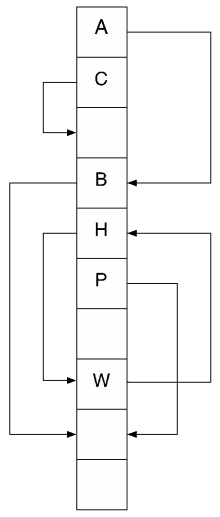
\includegraphics[height=8cm]{cuckoo.png}
\caption{Rappresentazione grafica di un cuckoo hashing}
\end{figure}

La ricerca pu\`o essere realizzata con poche righe di codice:

\begin{lstlisting}
int search(int x){
	if(T[h1(x)]==x) return h1(x);
	if(T[h2(x)]==x) return h2(x);
	return -1;
}
\end{lstlisting}

Per quanto riguarda invece la procedura di inserimento notiamo che le funzioni $h_1$ e $h_2$ vengono utilizzate in modo equivalente, non \`e rilevante quale utilizzare per prima nel confronto.

\begin{lstlisting}
void insert(int x){
	if(search(x) != -1) return;
	int pos = h1(x);
	for(int i = 0; i < n; i++){
		if(T[pos] == NULL) {T[pos] = x; return}
		swap(x, T[pos]);
		if (pos == h1(x)) pos = h2(x); else pos = h1(x);	
	}
	rehash;
	insert(x);
}	
\end{lstlisting}

Notiamo che pu\`o succedere che non riusciamo ad inserire un elemento all'interno del dizionario perch\'e si \`e venuto a creare un ciclo. Per renderci conto che ci troviamo in questa situazione effettuiamo il ciclo di inserimento per $n$ volte, nel caso in cui non siamo riusciti a sistemare tutti gli elementi, effettuato un \textsf{rehash()}, ovvero ricreiamo tutta la struttura.

\section{Analisi}

Per effettuare l'analisi del cuckoo hashing dobbiamo prima partire dal seguente Lemma:

\paragraph{Lemma} \emph{Prese due posizioni $i$ e $j$ ed una costante $c > 1$, se vale che $r \geq 2cn$ (ovvero che il nostro cuckoo hashing di fatto \`e un grafo molto sparso) allora vale che $$ \Pr(\exists \mbox{un cammino di lunghezza} \; l) \leq \frac{1}{c^{l}r}$$}

Ricordiamo che se immaginiamo il cuckoo hashing come un grafo, $r$ rappresenta il numero dei nodi e $n$ il numero degli archi.

\begin{proof}
La dimostrazione procede per induzione su $l$.

Per il caso $l=1$, se considero due posizioni $i$ e $j$ la probabilit\`a che esista un cammino fra queste due dipende strettamente dalla probabilit\`a che due elementi abbiamo $i$ e $j$ come possibili elementi (equivale a scegliere 2 posizioni su $r$ e si ripete l'operazione per due elementi).

Succede dunque che la probabilit\`a per due elementi risulta essere $\frac{2}{r^2}$, se invece considero tutti i possibilit elementi la probabilit\`a risulta $$\sum_{x \in S} \frac{2}{r^2} \leq \frac{2n}{r^2} \leq \frac{c^{-1}}{r}$$

Ricordiamoci che avevamo imposto che:$$r \geq 2cn \quad \mbox{ovvero} \quad \frac{r}{c} \geq 2n$$

Per il caso induttivo, assumiamo che esista:
\begin{enumerate}
\item Un cammino di lunghezza $l-1$ tra $i$ un elemento $k$
\item Un collegamento fra $k$ e $j$.
\end{enumerate}
Il primo punto pu\`o accadere, per ipotesi induttiva, con probabilit\`a $\frac{1}{c^{(l-1)}r}$ mentre il secondo pu\`o venire con probabilit\`a $\frac{1}{cr}$ per il caso base visto prima.

Se ne deduce che la probabilit\`a che esista un cammino di lunghezza $l$ fra due elementi risulta essere $$\frac{1}{c^l r^2} \leq \frac{1}{c^l r}$$
\end{proof}

Di fatto un \emph{bucket} in un cuckoo hashing \`e un cammino fra due nodi. Abbiamo dimostrato che due elementi finiscono nello stesso \emph{bucket} con probabilit\`a $O(\frac{1}{r})$ e al contempo che decresce esponenzialmente al crescere di $l$.

Possiamo dare un limite superiore alle operazioni necessarie per un generico elemento $x$, considerando la dimensione del bucket di $x$. Vediamo che la probabilit\`a di effettuare operazioni su $x$ risulta essere $O(1/r)$, sommiamo per tutti gli elementi in $S$ e vale che: $$|S| \cdot O(1/r) = O(1) \quad \mbox{dato che} \quad r \geq n \geq |S|$$

\section{Cicli}

Analizziamo adesso qual \`e la probabilit\`a che esista un ciclo fra due generici elementi.

Dato $S$ consideriamo una sequenza di $\varepsilon n$ inserimenti, con $\varepsilon > 0$ e piccolo, vediamo che possiamo considerare la probabilit\`a di avere un ciclo  su k con la probabilit\`a di avere un cammino da k a k (di lunghezza non fissata):

$$\Pr(\mbox{ciclo su k}) \leq \Pr(\exists \mbox{un cammino fra k e k}) = \sum_{l=0}^{n-1}(Lemma1) \leq \left(\sum_{l}\frac{1}{c^l r} \right) = O\left(\frac{1}{r}\right) \leq \frac{1}{(c-1)r}$$

Notare che prendiamo $r \geq 2c(1+\varepsilon)n$.

Per calcolare la probabilit\`a effettiva che ci sia un ciclo, consideriamo tutti i vertici:
$$ r \cdot \sum_{l}\frac{1}{c^l r} = r \cdot \frac{1}{(c-1)r} \leq \frac{1}{c-1} \leq \frac{1}{2}$$
Abbiamo utilizzato lo sviluppo della serie $x^l$ per arrivare a questo risultato. Qui potremmo utilizzare i chernoff bound per limitare questo risultato a piacimento.

\section{Re-hashing}

La probabilit\`a di fare un rehashing pu\`o essere maggiorato dalla probabilit\`a di avere un ciclo nel grafo.

Supponiamo ad esempio di scegliere la costante $c=3$:
\begin{enumerate}
\item Con probabilit\`a $1/2$ faccio 1 rehashing,
\item Con probabilit\`a $1/4$ faccio 2 rehashing,
\item Con probabilit\`a $1/8$ faccio 3 rehashing,
\item etc...
\item Con probabilit\`a $1/2^i$ faccio $i$ rehashing,
\end{enumerate}

Cerchiamo adesso di determinare il numero medio di rehashing che eseguo: $$\sum_{i=1}^{\infty}\frac{1}{2^i} \leq 2$$.

La maggiorazione risulta dallo schema seguente:
\begin{center}
\begin{tabular}{ccccl}
 & & & $\dots$ & $\longleftarrow \leq \dots$ \\
 & & & $1/16$ & $\longleftarrow \leq 1/8$ \\
 & & $1/8$& $1/16$ & $\longleftarrow \leq 1/4$ \\
 & $1/4$& $1/8$& $1/16$ & $\longleftarrow \leq 1/2$ \\
$1/2$ & $1/4$& $1/8$& $1/16$ & $\longleftarrow \leq 1$ \\
\end{tabular}
\end{center}

Sommando i numeri sulla sinistra possiamo notare che otteniamo una serie nota che converge a 2. Quindi in media ho 2 rehashing, nel caso ne avessi di pi\`u significa che ho scelto in modo sbagliato i parametri $a_i$ e $b_i$ delle mie funzioni hash.

Ogni rehashing costa $O(n)$ in tempo, ma risulta che il costo \emph{ammortizzato} del rehashing \`e $O(1)$.

\section{Cancellazione}

Analizziamo adesso il problema della cancellazione da un cuckoo hashing. Notiamo che il \emph{cluster} (ovvero l'insieme delle posizioni nelle quali si pu\`o trovare un elemento) \`e 2, quindi ritrovare la chiave per rimuoverla \`e relativamente semplice.

Il problema \`e che la struttura dati generata \`e randomizzata mentre l'operazione di cancellazione \`e deterministica.

\paragraph{Domanda} Una volta rimosso un elemento dal cuckoo hashing, riesco a scegliere altri $h'_1$ e $h'_2$ che ricreino la mia configurazione attuale?

\paragraph{Risposta} S\`i, scelgo $h'_1$ in modo che mappi gli elementi esattamente come sono posizionati adesso nella struttura, e scelgo $h'_2$ in modo libero.

\chapter{Filtri di Bloom}

I filtri di Bloom sono una struttura dati presentata negli anni '70 che permette la memorizzazione di un insieme di dati $S$ offrendo un notevole risparmi in termini di spazio, causando per\`o dei falsi positivi, ovvero rispondendo al test di appartenenza di un elemento all'insieme con \textsf{true} anche se l'elemento non appartiene all'insieme.

Sono utilizzati in quegli ambiti dove i falsi positivi non destano problemi, perch\`e la probabilit\`a che hanno di occorrere sia sufficientemente bassa, specialmente nel campo del networking, ad esempio nei router e nei proxy.

I filtri di bloom si basano sul seguente principio:
\newtheorem{bloom}{Bloom Filter Principle}
\begin{bloom}
When ever a list or set is used, and space is at premium, consider using a bloom filter if the effect of false positive can be mitigated.
\end{bloom}

\section{Definizione matematica}

Un filtro di bloom per memorizzare un insieme $S = \{x_1, x_2, \cdots, x_n\}$ \`e un vettore di $m$ bit che inizialmente sono settati tutti a 0.

Si scelgono inoltre in modo indipendente $h_1, \cdots, h_k$ funzioni hash da una famiglia di funzioni hash $H: S \rightarrow [m]$.

L'inserimento di un nuovo elemento avviene nel modo seguente:
\begin{verbatim}
INS(x)
    for(i=0; i<k; i++) T[hi(x)]=1;
\end{verbatim}
Si calcolano ovvero tutte le $k$ funzioni hash per il nuovo elemento, e si settano a 1 i bit nelle posizioni risultati dalle funzioni hash.

La ricerca viene avviene nel modo seguente:
\begin{verbatim}
SEARCH(X)
    j = 1
    while(j <= k && T[hj(x)] == 1)
        j++;
    return j > k;
\end{verbatim}
Si va dunque a verificare se tutti i bit nelle posizioni risultanti dal calcolo delle funzioni hash sull'elemento sono settati a 1.

Si vede facilmente che questa ricerca pu\`o generare dei falsi positivi, specialmente dopo sequenze di inserimenti abbastanza lunghe e per valori di $m$ piccoli.

Nell'immagine seguente \	`e presente un esempio di filtro di bloom: vediamo l'inserimento degli elementi $x, y, z$ e la ricerca sull'elemento $w$.

\begin{figure}
\centering
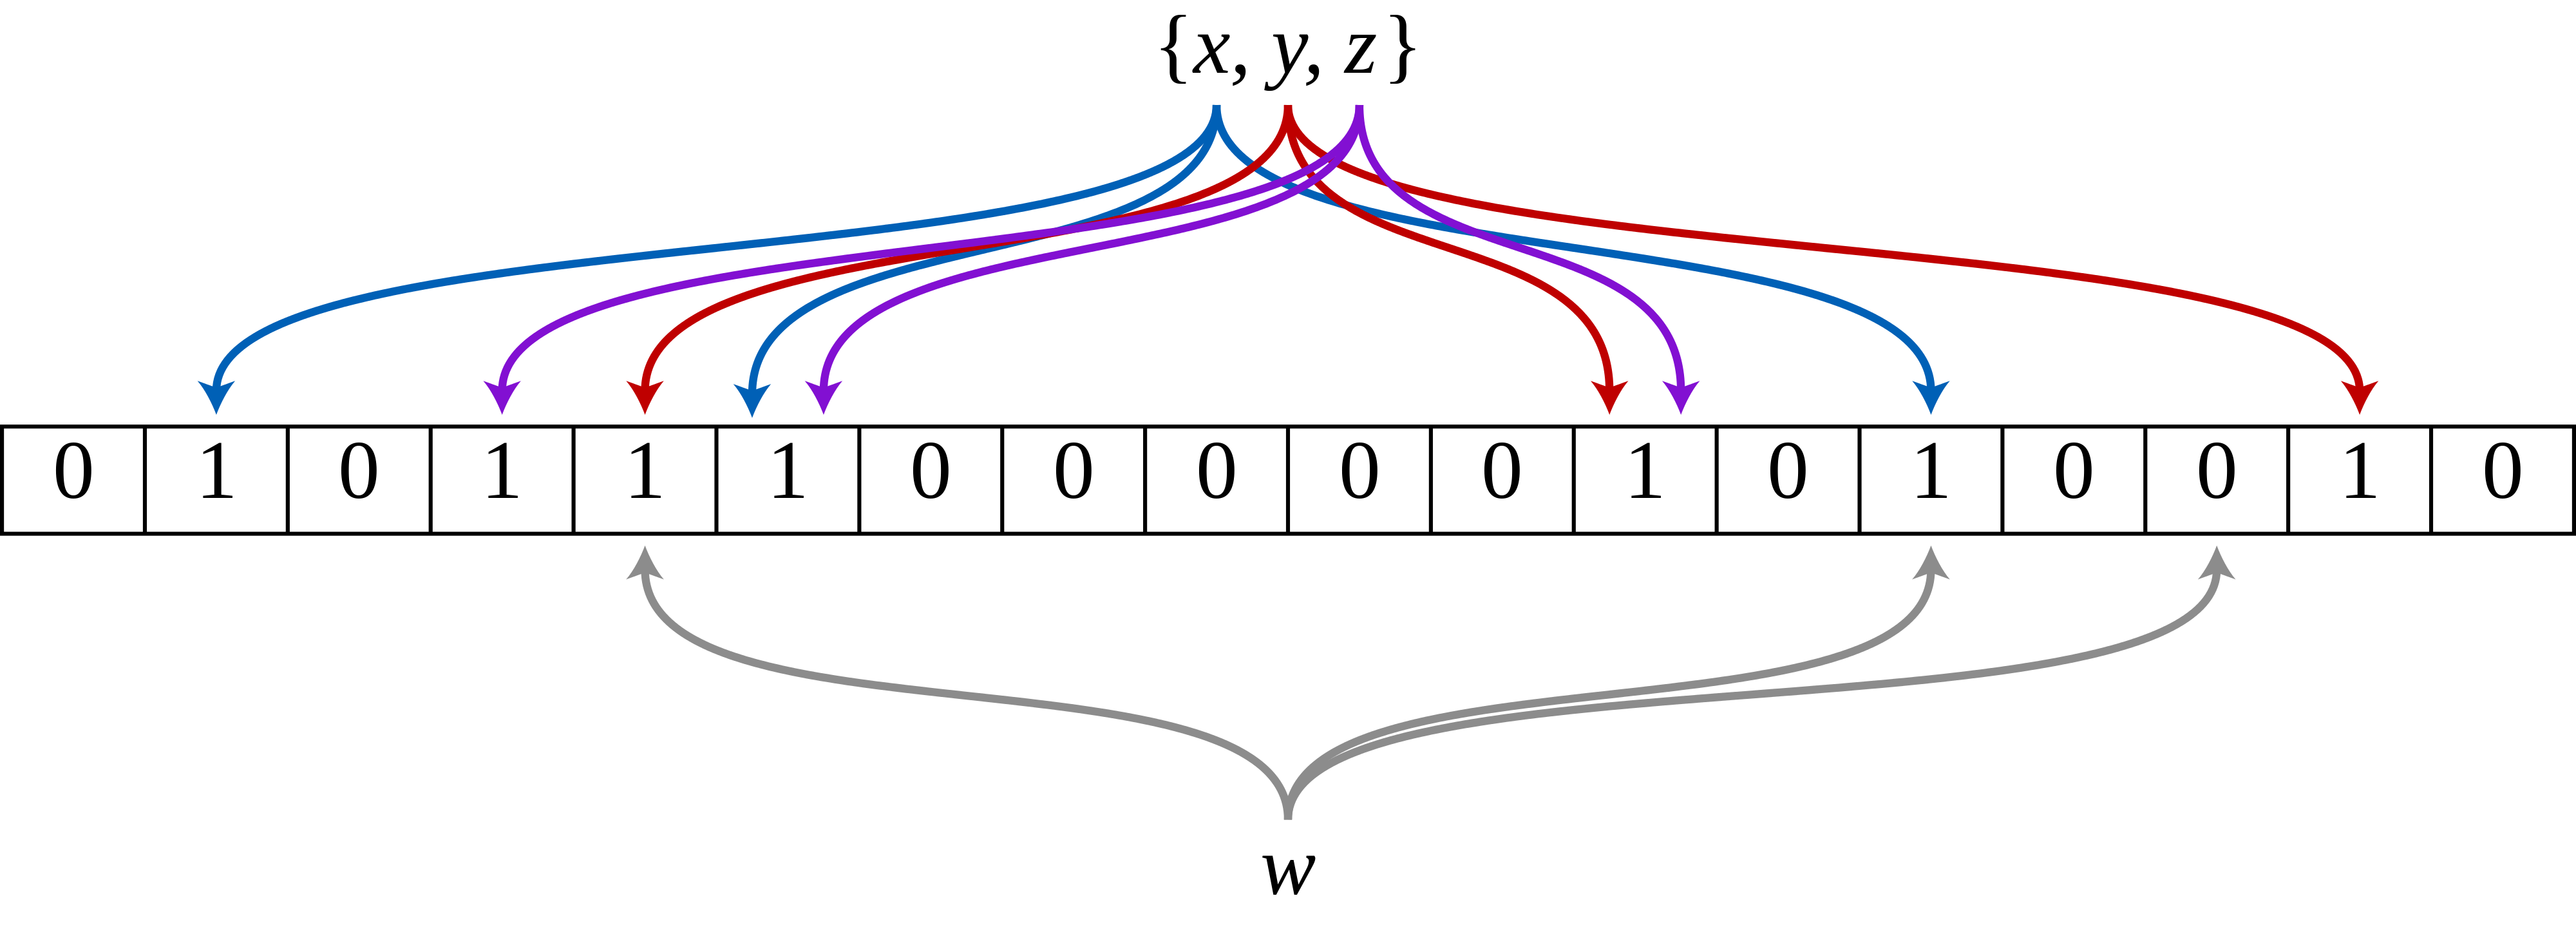
\includegraphics[height=4cm]{bloom.png}
\caption{Filtro di bloom con $m = 18$ e $k = 3$}
\end{figure}

\section{Analisi}

Vediamo facilmente che la probabilit\`a per uno specifico bit di essere a 1 \`e $1/m$. Allora la probabilit\`a per uno specifico bit di essere sempre a 0 dopo n inserimenti nel filtro di bloom pu\`o essere facilmente calcolato con il complementare come: $$p' = \left( 1 - \frac{1}{m}\right)^{kn}$$

Utilizzando uno sviluppo di Taylor ricordiamoci che possiamo esprimere $e^x$ come:$$e^x = 1 + x + \frac{1}{2}x^2 + \cdots$$

Quindi riscriviamo: $$p' = \left( 1 - \frac{1}{m}\right)^{kn} \approx e^{-kn/m} = p$$

Intuitivamente notiamo che su aumentiamo la dimensione della tabella, aumenta il numero di zeri. Se invece aumentiamo il numero delle funzioni hash, il numero di zeri diminuisce.

Consideriamo adesso il fattore di carico $\rho$ come il rapporto fra il numero di zeri e il totale degli elementi del filtro di bloom, risulta che il valore atteso per $\rho$ \`e $E(\rho) = p'$. La probabilit\`a di un falso positivo \`e dunque legata alla probabilit\`a di ottenere un 1 per le k funzioni hash di un elemento ovvero: $$(1 - \rho)^k \approx (1 - p')^k \approx (1 - p)^k$$

Lo sviluppo pu\`o essere visto anche come:
\begin{eqnarray}
\Pr(\mbox{false positive for y}) & = & \Pr( \forall j : T[h_j (y)] = 1) \nonumber \\
& = & \prod^{k}_{j = 1} \Pr(T[h_j (y)] = 1) \nonumber \\
& = & \prod^{k}_{j = 1} 1 - \underbrace{\Pr(T[h_j (y)] = 0)}_{p'} \nonumber \\
& = & (1 - p')^k \nonumber \\
& = & \left(1 - \left( 1 - \frac{1}{m}\right)^{kn}\right)^k
 \nonumber \\
& \approx & (1 - p)^k \nonumber \\ \nonumber \\
& = & \left(1 - e^{\frac{-kn}{m}}\right)^k \nonumber
\end{eqnarray}

Intuitivamente notiamo che aumentando $k$, aumenta la probabilit\`a di un falso positivo, mentre aumentando $m$, diminuisce la probabilit\`a di un falso positivo.

\subsection{Scelta dei parametri}

Avendo calcolato la probabilit\`a di un falso positivo, \`e possibile determinare una scelta ottima per il parametro k:

Consideriamo la derivata di $(1 - p)^k$, che si azzera per $$k = \ln 2 \cdot (m/n)$$
Cos\`i facendo la probabilit\`a di un falso positivo diventa $$(1/2)^k \approx (0.6185)^{m/n}$$

\subsection{Rimozione di un elemento}

La rimozione pu\`o essere complicata, soprattutto se l'unione dei bit relativi all'elemento e l'unione dei bit relativi a tutti gli altri elementi a intersezione non vuota.

Alternative possono essere:
\begin{enumerate}
\item Un algoritmo dove non si utilizzano bit, ma si utilizzano dei contatori, e si effettuano operazioni del tipo $T[h_j (x)]++$. Questa soluzione presenta per\`o un costo in spazio molto pi\`u elevato rispetto ai filtri di bloom classici. Si utilizzano $\log n$ bit (anche se con i chernoff bound si pu\`o dimostrare che si utilizza meno spazio).
\item Un algoritmo dove il vettore \`e separato in settori di dimensione $m/k$.
\end{enumerate}

\section{Operazioni Booleane}

Supponiamo di avere due filtri di bloom $S_1$ e $S_2$, se vogliamo sapere se un elemento appartiene all'unione dei due insiemi, \`e sufficiente considerare il filtro di bloom $S_1 \vee S_2$, dove i bit sono messi in \textsf{OR} fra di loro.

Inoltre \`e possibile stimare la dimensione dell'intersezione di due insiemi nel modo seguente: $$|S_1 \cup S_2| = \frac{S_1 \odot S_2}{k} $$ dove ${S_1 \odot S_2}$ rappresenta il prodotto scalare fra i due filtri di bloom coinvolti.

\section{Compressione}

Ai fini della compressione \`e conveniente realizzare un filtro di bloom pi\`u grosso, ma che contiene pi\`u 0, in modo che riuscir\`o a comprimerlo meglio, e trasmetter\`o meno bit.

\chapter{Algoritmi Randomizzati}

In questa sezione vedremo alcuni algoritmi randomizzati, che sfruttano il ruolo della casualit\`a per cercare di rendere trascurabili le condizioni sfavorevoli dell'algortimo.

Considereremo un'analisi di tipo avversariale, dove consideriamo l'esistenza di un avversario che, con maliziosit\`a, cerca di presentarci sempre le condizioni sfavorevoli. In questo contesto cercheremo di usare la casualit\`a a nostro favore.

Consideriamo il caso del quicksort:

\section{Il quicksort}

L'algoritmo di ordinamento del quicksort \`e descritto nel codice seguente:
\begin{lstlisting}
void QuickSort(A, sx, dx){
	if(sx < dx){
		pivot = random(sx..dx);
		px = distribution(A, sx, pivot, dx);
		QuickSort(A, sx, px-1);
		QuickSort(A, px+1, dx);
	}
}
\end{lstlisting}

Risulta evidente che se il pivot venisse scelto come uno dei due estremi dell'array ci troveremo nella situazione peggiore.
La chiamata ricorsiva costerebbe infatti $$T(n) \leq T(n-1) + cn$$ E quindi l'algoritmo avrebbe un costo quadratico $$T(n) = O(n^2)$$

Proviamo ad effettuare un'analisi cercando di calcolare il tempo di esecuzione atteso che sappiamo essere $n\log n$:
$$\underbrace{E[\mbox{runningtimeQS}]}_{\tilde{T}} = O(n\log n)$$

Partiamo dall'ipotesi che la nostra funzione \textsf{random()} restituisca numeri distribuiti in modo uniforme fra sx e dx.

A seguito dell'invocazione della funzione \textsf{distribution()} abbiamo che il nostro px risulta distribuito in modo uniforme fra sx e dx (proprio come per la funzione \textsf{random()}). Vale dunque che una scelta casuale di pivot equivale ad una scelta casuale di px.

Adesso supponiamo di dividere il nostro array in 4 zone\footnote{L'analisi vale per qualunque numero $i \geq 3$} contigue, dato che il nostro px \`e equidistribuito possono succedere 2 casi:

\begin{enumerate}
\item px si trova in una delle due zone interne, ci\`o pu\`o accadere con probabilit\`a $\frac{1}{2}$. Questo \`e per noi un caso fortunato.
\item px si trova in una delle due zone esterne, ci\`o pu\`o accadere con probabilit\`a $\frac{1}{2}$. Questo \`e per noi un caso sfortunato.
\end{enumerate}

Nel primo caso, consideriamo il caso pessimo dove px si trova in uno dei due estremi delle zone, allora vale che: 
$$\tilde{T}(n) = \tilde{T}\left(\frac{1}{4}n\right) + \tilde{T}\left(\frac{3}{4}n\right) + cn$$
Mentre nel secondo caso vale che:$$\tilde{T}(n) \leq \tilde{T}(n-1) + cn = O(n^2)$$

Facciamo la media pesata dei due termini e risolviamo:
$$\tilde{T}(n) \leq \frac{1}{2}\left[\tilde{T}\left(\frac{1}{4}n\right) + \tilde{T}\left(\frac{3}{4}n\right) + \tilde{T}(n-1)\right] + cn$$

$$\tilde{T}(n) \leq \frac{1}{2}\left[\tilde{T}\left(\frac{1}{4}n\right) + \tilde{T}\left(\frac{3}{4}n\right) + \tilde{T}(n)\right] + cn$$

$$2\tilde{T}(n) \leq \left[\tilde{T}\left(\frac{1}{4}n\right) + \tilde{T}\left(\frac{3}{4}n\right) + \tilde{T}(n)\right] + 2cn$$

$$\tilde{T}(n) \leq \left[\tilde{T}\left(\frac{1}{4}n\right) + \tilde{T}\left(\frac{3}{4}n\right) \right] + 2cn$$

$$\tilde{T}(n) = O(n \log n)$$

Vediamo dunque che con una scelta casuale equamente distrubuita del pivot riusciamo ad evitare di finire sempre nel caso sfortunato, ed abbiamo un algoritmo che costa cos\`i  $O(n \log n)$.

\section{Le skiplist}

Le \emph{skiplist} (o liste a saltelli) sono delle liste speciali che permettono di fare operazioni di ricerca su liste in un tempo medio di $O(\log n)$.

In questa struttura dati, proprio come nel quicksort, il caso svolge un ruolo determinante per avere un tempo medio logaritmico.

Le \emph{skiplist} si costruiscono in questo modo: partendo da una lista ordinata di $n$ elementi, si creano delle repliche della lista in modo che ogni elemento in posizione $i$ della lista sia presente nelle $r_i$ liste a lui superiore, dove $2^{r_i}$ rappresenta la massima potenza del 2 che divide $i$. Il numero delle liste \`e dato dal massimo numero di $r_i+1$ e vale che $h = O(\log n)$.

Il problema sussiste nel momento in cui si vuole aggiungere un nuovo elemento, \`e infatti semplice trovare il luogo adatto dove inserire il nuovo elemento, per\`o per mantenere le propriet\`a della \emph{skiplist} si dovrebbe ricostruire tutta la struttura.

Si preferisce piuttosto di decidere in modo casuale in quali liste inserire un nuovo elemento: lanciamo una moneta (quindi un evento casuale che ha probabilit\`a $\frac{1}{2}$) e continuiamo a lanciarla fin quando otteniamo testa, non appena otteniamo una croce ci fermiamo. Supponendo di aver ottenuto croce dopo $i$ lanci, allora replichiamo l'elemento nelle $i-1$ liste superiori\footnote{Questo procedimento pu\`o essere simulato con una funzione \textsf{random()} che restituisce 1 o 0 in modo equidistribuito.}. Il costo di questa operazione risulta essere $O(\log n)$.

Dato che i lanci della moneta sono indipendenti, notiamo che la probabilit\`a che un elemento sia presente nella $i-\mbox{esima}$ lista risulta essere $\frac{1}{2^i}$.

\subsection{Ricerca nelle \emph{skiplist}}

Vediamo che la ricerca di un elemento $k$ \`e proporzionale a $O(T(l))$, dove $T(l)$ \`e il numero di elementi che vengono incontrati a partire dalla lista di altezza $l$ fino al predecessore di $k$ nella lista $L_0$.

Osserviamo che il percorso inverso di ricerca \`e a gradini, per cui per un generico elemento $e \in L_l$ possono succedere due avvenimenti:
\begin{enumerate}
\item Il percorso proviene dall'elemento al livello inferiore, dove il costo risulta essere $T(l-1)$. Ci\`o pu\`o avvenire con probabilit\`a $\frac{1}{2^i}$, dato che \`e la stessa probabilit\`a con cui abbiamo effettuato i lanci della nostra moneta per verificare se replicare o meno un elemento.
\item Il percorso proviene dall'elemento a destra, dove il costo medio risulta essere $T(l)$, ci\`o vuol dire che $e$ non ha una copia al livello superiorie. Ci\`o avviene con probabilit\`a uguale a $\frac{1}{2^i}$, ovvero un lancio dove \`e uscito croce.
\end{enumerate}

Risulta allora che: $$T(l) \leq \frac{1}{2}T(l) + \frac{1}{2}T(l-1) + c'$$
$$T(l) \leq T(l-1) + c'$$
Quindi:
$$T(h) = O(h) = O(\log n)$$

\subsection{Cancellazione nelle \emph{skiplist}}

Per quanto riguarda la cancellazione \`e sufficiente rimuovere l'elemento dalla struttura, e non si perde la casualit\`a della struttura.

Rimuovendo un elemento si vede infatti facilmente che \`e possibile ricreare la struttura senza quell'elemento in modo casuale.

\section{I Random Binary Search Trees}

I Random Binary Search Trees (RBST) sono un'altra struttura dati che sfrutta la casualit\`a per generare degli alberi binari di ricerca. Essi mantengono le stesse propriet\`a dei Binary Search Tree.

L'altezza di un BRST \`e in media logaritmica, rendendo il costo delle operazioni di inserimento e ricerca in media logaritmici.

I RBST si basano su una propriet\`a fondamentale: data una sequenza di $n$ chiavi $K$, ogni chiave pu\`o essere radice del RBST con probabilit\`a $\frac{1}{n}$.

\subsection{Inserimento in un RBST}

Considerando la propriet\`a precedente, nel momento in cui voglio inserire un nuovo elemento, devo prima testare se questo nuovo elemento pu\`o essere la radice del mio RBST. Questo pu\`o avvenire con probabili\`a $\frac{1}{n+1}$, provo quindi a generare un numero casuale da 0 a n:

\begin{itemize}
\item Se esce 0, allora l'elemento sar\`a radice, e collego il vecchio albero come figlio sinistro/destro a seconda del valore. Dopodich\'e eseguo una procedura \textsf{split()} per effettuare un taglio del vecchio RBST in modo da redistribuire i nodi\footnote{Vedi articolo di Martizen, Rouna, pag. 293}.
\item Se esce $k \neq 0$ allora itero su uno dei due sottoalberi (che sono anch'essi dei RBST), secondo il valore 
\end{itemize}, 

Segue l'algoritmo di inserimento nel RBST:

\begin{lstlisting}
rbst insert(int x, rbst T){
	int n, r;
	
	n = T->size;
	r = random(0, n);
	
	if (r == n)
		return insert_at_root(x, T);
	if (x < T->key)
		T->left = insert(x, T->left);
	else
		T->right = insert(x, T->right);
	return T;
}
\end{lstlisting}

%Esempio grafico??%

\chapter{Compressione Dati}

Gli algoritmi di compressione permettono di comprire un dato S in un dato Z con un numero inferiore di bit.

Esistono due famiglie di algoritmi di compressione:
\begin{description}
\item[algoritmi loseless] ovvero che permettono di comprimere e di decomprimere senza perdita di informazioni
\item[algoritmi lossy] ovvero che comportano perdita di informazioni durante il processo di compressione.
\end{description}

Per studiare gli algoritmi loseless dobbiamo introdurre il concetto di entropia.

\section{Entropia}

L'entropia, secondo quanto definito da Shannon, rappresenta la quantit\`a di incertezza presente in un segnale.

Supponiamo $ S \in \Sigma^n $ dove $S$ rappresenta una stringa dell'alfabeto $\Sigma$ di lunghezza $n$. Contiamo le occorrenze di ogni simbolo distinto in questo modo: $$ n_c = \{i : 0 \leq i \leq n-1  |  S[i] o determine the probability, divide by .
[edit]= c\}$$ e definiamo le probabilit\`a di occorrenza di ogni singolo simbolo come $ p_c = \frac{n_c}{n}$, definiamo allora l'entropia come segue: $$ H(s) = - \sum_{c \in \Sigma} p_c \log p_c = \sum_{c \in \Sigma} p_c \log \frac{1}{p_c}$$

Grazie alla definizione di entropia di Shannon \`e possibile enunciare il primo teorema di Shannon:

\newtheorem{shan1}{Primo Teorema di Shannon}
\begin{shan1}
Per trasmettere un segnale $S$ di lunghezza $n$ senza perdita di informazione sono necessari almeno $nH(s)$ bit.
\end{shan1}

Nell'ambito della complessit\`a risulta interessante considerare anche la complessit\`a di Kolmogorov.

\section{Complessit\`a di Kolmogorov}

Sia $F$ un formal computation model allora definiamo la Complessit\`a di Kolmogorov ($K_{F}(S)$) come il pi\`u breve programma scritto in $F$ che riesce a generare $S$.

Ovviamente $K_{F}(S)$ non \`e calcolabile, e risulta invariante rispetto $F$, a meno di una costante, vale infatti che:$K_{F'}(S) = K_{F}(S) + \Theta(1)$

Notiamo che l'entropia definita da Shannon \`e relativa ad una sorgente di stringhe, mentre invece la complessit\`a di Kolmogorov \`e relativa ad una singola stringa.

\section{Elias Coding}

Vediamo adesso due codifiche proposte da Peter Elias nel '75, il $\gamma-code$ e il $\delta-code$.

I codici di Elias sono codici a codifica variabile, ovvero codici che assegnano quantit\`a di bit differente ad ogni simbolo ed inoltre sono codici \emph{prefix-free}, ovvero non pu\`o accadere che un simbolo venga codificato con $k$ e un altro simbolo venga codificato con $k'$ tale che $k'$ \`e prefisso di $k$.

\subsection{Il $\delta-code$}

Per codificare un numero $x$ con il suo $\delta-code$ si eseguono i seguenti passi:
\begin{enumerate}
\item Si calcola la pi\`u grande potenza del 2 contenuta dentro $x$ ovvero $c(x) = \lceil \log_2 (x) \rceil$,
\item Si codifica $c(x)$ in unario, ovvero lo si rappresenta come una sequenza di $c(x)-1$ zeri seguiti da un uno ($0^{c(x)-1}1$),
\item Accodiamo la rappresentazione binaria di $x$ senza il primo uno (che \`e stato inserito al punto precedente). 
\end{enumerate}

Abbiamo cos\`i ottenuto la codifica che risulta occupare $2 \lfloor \log_2 (x) \rfloor + 1$ bit.

Il $\delta-code$ viene utilizzato per codificare sequenze di numeri di cui non \`e noto a priori l'upper bound oppure sequenze dove i numeri pi\`u piccoli sono pi\`u frequenti (dato che la loro rappresentazione \`e pi\`u breve).

\subsection{Il $\gamma-code$}

Il $\gamma-code$ procede in modo simile al $\delta-code$ visto poco fa:

\begin{enumerate}
\item Si calcola la pi\`u grande potenza del 2 contenuta dentro $x$ ovvero $c(x) = \lceil \log_2 (x) \rceil$,
\item Si calcola $\delta(c(x)+1)$
\item Accodiamo la rappresentazione binaria di $x$ senza il primo uno (che \`e stato inserito al punto precedente). 
\end{enumerate}

Il $\gamma-code$ occupa cos\`i $\lfloor \log_2 (x) \rfloor + 2 \lfloor \log_2 (\lfloor \log_2 (x) \rfloor+1) \rfloor + 1$

\section{Codifica di Hufmann}

La codifica di Huffman \`e stata realizzata nel 1952 da David Huffman, \`e una codifica a lunghezza variabile, \emph{prefix-free} ed \`e una codifica che assegna codifiche di lunghezza minore ai simboli pi\`u frequenti.

Si pu\`o dimostrare inoltre che la codifica di Hufmann assenga le codifiche pi\`u brevi ai singoli pi\`u frequenti rispetto ad altre codifiche.
Vale ovvero che il termine $$ \sum_{c\in\Sigma}l_{c}p_c$$ dove $l_c$ rappresenta la lunghezza della codifica del simbolo $c$ e $p_c$ la sua frequenza nella stringa viene minimizzato, e vale $nH(S) + n$.

\subsection{Descrizione della codifica}

La codifica opera in questo modo:
\begin{enumerate}
\item Calcola le frequenze per ogni simbolo della stringa e li inserisce in una coda.
\item Fin quando la coda non \`e vuota:
\begin{enumerate}
\item Considera i due elementi a frequenza minore e li rimuove dalla lista,
\item Crea un albero usando come figli i due elementi e inserendo come padre un nuovo elemento.
\item Si inserisce nella lista il padre che ha come frequenza la somma delle frequenze dei figli.
\end{enumerate}
\item Una volta generato l'albero si assegna una codifica binaria ad ogni numero (ad esempio 0 se si sceglie il ramo sinistro e 1 se si sceglie il ramo destro).
\end{enumerate}

Come si vede l'albero viene generato partendo dal basso ed inserendo prima gli elementi meno frequenti che quindi avranno cammini pi\`u lunghi e di conseguenza codifiche pi\`u lunghe.

\paragraph{Esempio}

Vogliamo codificare la stringa \emph{abracadabra}. L'albero risultate \`e:

\Tree [.$\bullet$ a [.$\bullet$ b [.$\bullet$ [.$\bullet$ c d ] r ] ] ]

Possiamo dunque codificare i vari caratteri nel modo seguente: $a = 0$ , $b = 10$, $c = 1100$, $d = 1101$, $r = 111$.

\section{Codifica LZ77/LZ78}

Gli algoritmi LZ77 ed LZ78 sono due algoritmi di compressione loseless cercano di sfruttare la ricerca di sottostringhe ricorrenti all'interno dello stream al fine di ridurre la quantit\`a di dati da memorizzare.

\subsection{LZ77}

La prima codifica, LZ77, analizza lo stream in modo sequenziale va a cercare per ogni simbolo se vi sono delle occorrenze passate. Per ogni simbolo codifica una tripla cos\`i fatta: $$(i-i', |\alpha|, c)$$ dove $$i-i'$$ rappresenta la distanza dal simbolo attuale e l'occorrenza passata\footnote{Si noti che viene memorizzata la posizione relativa e non assoluta, dato che questo algoritmo pu\`o essere utilizzato anche per file di grandi dimensioni}, $|\alpha|$ rappresenta la dimensione della sottostringa, e $c$ rappresenta il prossimo carattere incontrato.

Ad esempio la stringa \emph{abracadabra} viene codificata cos\`i:$$S = |a|b|r|ac|ad|abra\$ $$
$$ Z = (0,0,a),(0,0,b),(0,0,r),(3,1,c),(2,1,a),(7,4,\$)$$

Oppure la stringa \emph{ababababab} viene codificata cos\`i:$$S = a|b|abababab\$ $$
$$ Z = (0,0,a),(0,0,b),(2,8,\$)$$

\subsection{LZ78}

La seconda codifica, LZ78, usa invece un dizionario per memorizzare le sottostringhe incontrate. Risulta per\`o leggermente meno efficente della codifica LZ77.

%ESEMPIO?%

\part{Hard Problems}

\chapter{R-Approssimazione}

In questo capitolo vedremo un modo per approssimare problemi complessi, ad esempio problemi appartenendi alla classe \textsf{NP-Hard}. Per i problemi in questa classe si conoscono degli algoritmi per risolverli in tempo \textsf{EXP} ma non si conoscono algortimi che li risolvono in tempo \textsf{P}.

Molti problemi appartengono alla classe \textsf{NP-Hard}, quali ad esempio problemi legati ai trasporti, o all'economia. Per questo motivo si cercano algoritmi che approssimino le soluzioni dei problemi in tempo inferiore ad \textsf{EXP}.

Definiamo la classe \textsf{NP} come $$\mbox{NP} = \{ \pi \in \{0,1\}^* \; : \exists \mbox{poly} \; p(), V : $$
\begin{eqnarray}
1) & \forall x \in \{0,1\}^*, \;  x \in \pi & \Leftrightarrow & \exists y \in \{0,1\}^*, |y| = p(|x|), V(x,y) = 1 \nonumber \\
2) & \forall x \in \{0,1\}^*, \;  x \not\in \pi & \Leftrightarrow & \forall y \in \{0,1\}^*, V(x,y) = 0 \nonumber \} \\
\end{eqnarray}

Fra i possibili problemi all'interno di una classe si possono definire due tipi di problemi:
\begin{itemize}
\item Problemi decisionali,
\item Problemi di ottimizzazione.
\end{itemize}

Nei problemi decisionali si tratta di restituire ad una domanda di appartenenza o meno ad un insieme, quindi le possibili risposte possono essere \textsf{true} o \textsf{false}. Nei problemi di ottimizzazione si cerca una soluzione che minimizzi/massimizzi una funzione costo/beneficio.

In particolare definiamo la funzione costo/beneficio come: $$C : \pi \rightarrow \mathbb{R}$ E distinguiamo due tipi di problemi di ottimizzazione: i problemi di minimo, in cui cerchiamo di minimizzare il costo, cerchiamo dunque $$\mbox{arg} \min_{i \in \pi} C(i)$$ Mentre nei problemi di massimo cerchiamo di massimizzare il beneficio, ovvero: $$\mbox{arg} \max_{i \in \pi} C(i)$$.

\subsection{Problema del Commesso Viaggiatore}

Il problema del commesso viaggiatore (\emph{TSP - Travel Salesman Person}) \`e un problema di minimo in cui, dato un insieme di $N$ citt\`a tra cui sono definite le distanze $D[]$, si cerca un Tour (una sequenza) di citt\`a che attraversi tutte le citt\`a tale che minimizzi: $$C(i) = (\sum_{i} D(T[i], T[i+1])) + D(T[n], T[0])$$

Possiamo anche definire la versione decisionale, in modo da decidere se $\exists$ un Tour tale che $C(T) < k$, dove $k$ \`e una costante data.

\subsection{Problema del Maximal Independent Set}

\end{document}
